\documentclass{article}
\linespread{1.3}
\usepackage[margin=50pt]{geometry}
\usepackage{amsmath, amsthm, amssymb, amsthm, tikz, fancyhdr, graphicx}
\pagestyle{fancy}
\renewcommand{\headrulewidth}{0pt}
\newcommand{\changefont}{\fontsize{15}{15}\selectfont}

\fancypagestyle{firstpageheader}
{
  \fancyhead[R]{\changefont Michael Huang \\ CFRM 420 \\ Homework 4}
}

\begin{document}

\thispagestyle{firstpageheader}

\section*{1.}
{\Large 

Let $\{Z_t\} \sim \text{GWN}(0, 1).$ Let $Y_t = Z_tZ_{t-1}, t \in \mathbb{Z} $

% \begin{verbatim}
%   Text enclosed inside \texttt{verbatim}
%   environment 
%   is printed directly 
%   and all \LaTeX{} commands are ignored.
% \end{verbatim}

% \framebox[1.1\width]{\textbf{answer}}

\subsection*{(a)}

We know that by definition, $Z \sim \text{WN}(0, 1)$, that is, $Z \sim \text{IID}(0, 1)$ and $Z_t \sim \text{N}(0, 1)$. 
To show that $\{Y_t\}_{t \in \mathbb{Z}}$ is white noise, we need to prove the following conditions: \\ \\ 
$\mathbb{E}[Y_t] = 0$. We know that the expectation of two IID variables is their product, so we can show that \\
$\mathbb{E}[Y_t] \\ = \mathbb{E}[Z_tZ_{t-1}] \\ = \mathbb{E}[Z_t] \cdot \mathbb{E}[Z_{t-1}] \\ = 0 \cdot 0 = 0$ \hfill since $Z$ is Gaussian white noise. \\ \\ 
$\text{Var}(Y_t) = \sigma^2 = 1$. We can calculate this by definition as well: \\
$\text{Var}(Y_t)$ \\
$= \text{Var}(Z_tZ_{t-1})$ \\ 
$= \mathbb{E}(Z_{t-1})^2\text{Var}(Z_t) + \text{Var}(Z_{t-1})\mathbb{E}[Z_t^2]$ \\
$= 0^2 \cdot 1 + 1 \cdot \text{Var}(Z_t) + [\mathbb{E}(Z_t)]^2$ \hfill by definition of $\mathbb{E}[X^2]$ \\
$= 0 + 1 \cdot  1 + 0^2$ \\
$= 1$ \\ \\
$\text{Corr}(Y_k, Y_l) = 0$ for all $k \neq l$. We know by definition that \\
$\text{Corr}(Y_k, Y_l)$ \\ 
$= \frac{\text{Cov}(Y_k, Y_l)}{\sqrt{Var(Y_k)Var(Y_l)}}$ \\
$= \frac{\text{Cov}(Z_kZ_{k-1}, Z_lZ_{l-1})}{\sqrt{Var(Z_kZ_{k-1})Var(Z_kZ_{k-1})}} $ \\ 
$= \frac{\text{Cov}(Z_kZ_{k-1}, Z_lZ_{l-1})}{\sqrt{1 \cdot 1}} $ \hfill as we previously showed \\ 
$= \frac{\mathbb{E}[Z_kZ_{k-1}Z_lZ_{l-1}] - \mathbb{E}[Z_kZ_{k-1}]\mathbb{E}[Z_lZ_{l-1}]}{\sqrt{1}} $ \hfill by definition of covariance \\ 
$= \frac{0 \cdot 0 \cdot 0 \cdot 0 - (0 \cdot 0) \cdot (0 \cdot 0)}{\sqrt{1 \cdot 1}
} $ \hfill as we previously showed and by definition \\
$= \frac{0}{1} = 0.$ \\ \\ 
In proving all these conditions, we have shown that $\{Y_t\}_{t \in \mathbb{Z}}$ is white noise.

\subsection*{(b)}

If $\{Y_t\}_{t \in \mathbb{Z}}$ were an IID sequence, we could calculate this using definition of expectation:
$\mathbb{E}[Y_t^2Y_{t-1}^2]$ \\ 
$= (\text{Var}(Y_t) + \mathbb{E}[Y_t]^2) \cdot (\text{Var}(Y_{t-1}) + \mathbb{E}[Z_{t-1}]^2)$ \\
$= (1 + 0^2) \cdot (1 + 0^2)$ \hfill by definition of $Y_t, Y_{t-1}$ \\ 
= 1. \\ \\ 
However, we can see that \\
$\mathbb{E}[Y_t^2Y_{t-1}^2]$ \\
$= \mathbb{E}[Z_t^2Z_{t-1}^2Z_{t-1}^2Z_{t-2}^2]$ \\
$= \mathbb{E}[Z_t^2Z_{t-1}^4Z_{t-2}^2]$ \\
$= \mathbb{E}[1 \cdot Z_{t-1}^4 \cdot 1]$ \hfill as we previously calculated \\
$= \mathbb{E}[Z_{t-1}^4]$ \\ 
% check this later
$= 3 * 1 = 3$ \hfill by definition \\ 
which we can clearly see does not equate. 

\newpage

\subsection*{(c)}

We plot this in R: 
\begin{figure}[h!]
  \centering
  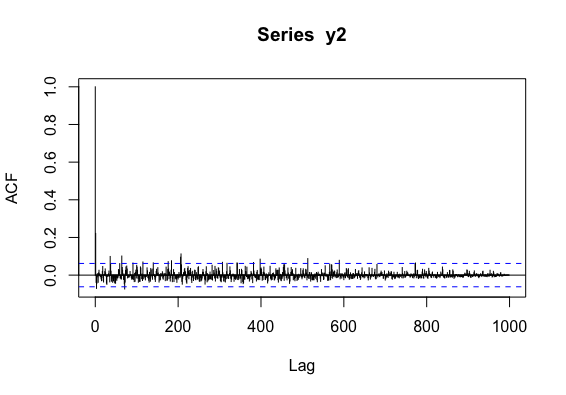
\includegraphics[width=500pt]{hw4_1c.png}
\end{figure}

\newpage

}

\section*{2.}
{\Large

\subsection*{(a)}



\subsection*{(b)}



\subsection*{(c)}



\subsection*{(d)}



\subsection*{(e)}

}

\end{document}